\section{Phenomenology of the MSSM}
\begin{frame}{How to test the MSSM?}
\addtocounter{framenumber}{-1}
\begin{figure}
	\centering 
	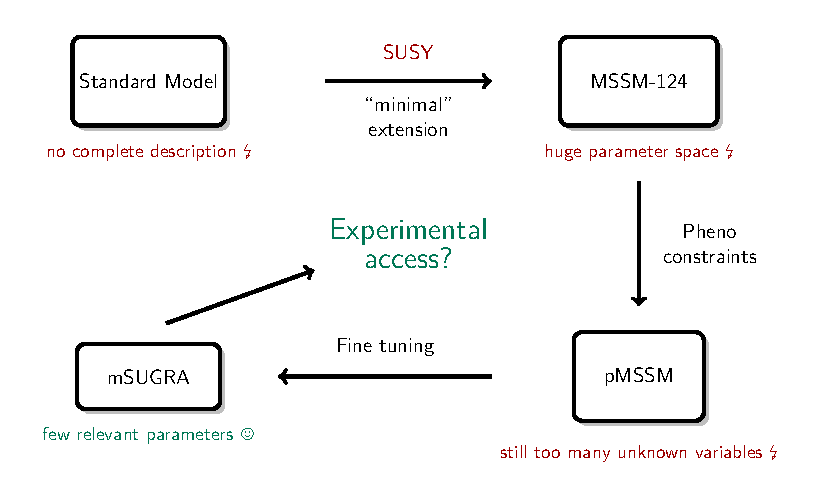
\includegraphics[scale = 0.9]{figures/overview}
\end{figure}
\end{frame}


\begin{frame}{Some Observations }
This huge additional parameter space in general comes with some severe problems :\\[1em]
\begin{minipage}{0.7\textwidth}
	
\end{minipage}
\begin{minipage}{0.29\textwidth}
	\begin{figure}
	\centering
		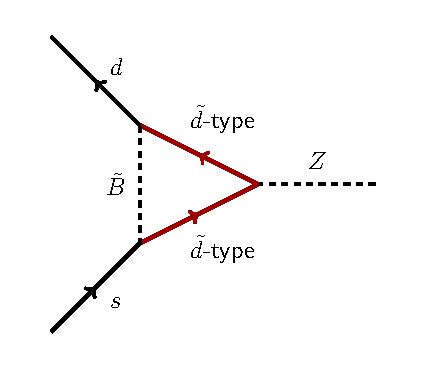
\includegraphics[scale = 0.6]{figures/fcnc_diagram}
	\end{figure}
\end{minipage}

For all of the above mentioned problems we have rather strict experimental bounds, for example:\\[1em]
Want to avoid contributions to \alert{electric dipole moments} $\implies$ complex phases of the gaugino mass parameters, $A$-parameters and $ \abs{\mu}$ $\lesssim  10^{-2} - 10^{-3}$ for TeV-ish sfermion and gaugino masses \cite{Fischler1992}.
\end{frame}

\begin{frame}{General Requirements}
We use these phenomenological constraints to define the \alert{phenomenological MSSM} (pMSSM) \cite{MSSMGroup1998}:\\[1em]
\begin{itemize}
	\item  No additional sources of CP-violation $\implies$ all phases in the soft-SUSY-breaking potential  zero \\[1em]
	\item No FCNCs $\implies$ simple, diagonal structure of the sfermion and trilinear coupling matrices\\[1em]
	\item First and second generation universality $\implies$ soft-SUSY-breaking scalar masses + trilinear couplings\footnote{Usually they are just set to zero for the first two generations\\} $A^{u}$, $A^d$ and $A^\ell$  are the same for the first two generations\\[2em]
\end{itemize}
 In addition, for different regions of the parameter space, one can use even more severe constraints\footnote{In actual experiments only very simplified models with two or three parameters are tested.}!
\end{frame}

\begin{frame}{Which Parameters do we need?}
This already reduces the number of relevant parameters by a large amount, a summary is given below:\\[1em]
\begin{itemize}
	\pause
	\item $\tan\beta = v_u/v_d$, the ratio of the VEVs in the two-Higgs doublet model\\[1em]
	\pause
	\item $m_{A}^2 = 2m_{12}^2  / \operatorname{sin} 2\beta$, the mass of the pseudoscalar Higgs boson\\[1em]
	\pause
	\item $M_{1}$, $M_{2}$ and $M_{3}$, the bino, wino and gluino masses\\[1em]
	\pause
	\item $\mu$, the Higgs-higgsino mass parameter\\[1em]
	\pause
	\item $m_{\tilde{q}}$, $m_{\tilde{u}_R}$, $m_{\tilde{d}_R}$, $m_{\tilde{\ell}}$ and $m_{\tilde{e}_R}$, the first/second generation sfermion masses\\[1em]
	\pause
	\item $m_{\tilde{Q}}$, $m_{\tilde{t}_R}$, $m_{\tilde{b}_R}$, $m_{\tilde{L}}$ and $m_{\tilde{\tau}_R}$, the third generation sfermion masses\\[1em]
	\pause
	\item $A^{t}$, $A^{b}$ and $A^{\tau}$, the third generation trilinear couplings\\[1em]
\end{itemize}
In total we are left with \alert{19 additional parameters} in the pMSSM.
 \end{frame}
 
 \begin{frame}{What about SUSY-breaking?}
 \begin{itemize}
 	\item The MSSM-124 fails to explain the fundamental origin of the SUSY-breaking parameters.\\[1em]
 	\item \textbf{Last talks:} Gauge- and gravity-mediated SUSY breaking may provide a way around!\\[1em]
  	\item The phenomenon of \alert{gauge coupling unification} hints at a simpler structure of the MSSM at\\ high energies.\\[1em]
 \end{itemize}
\begin{figure}
	\centering
	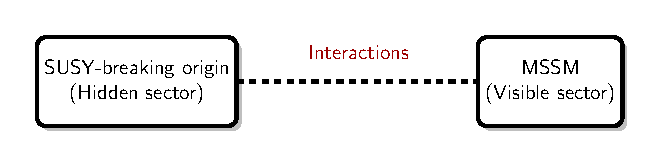
\includegraphics[scale= 1.1]{figures/susy_breaking}
	\caption{Gravity-mediated SUSY-breaking in the hidden sector\footnote{Figure inspired by the visualization in: \tiny\url{https://www.thphys.uni-heidelberg.de/~plehn/includes/bad_honnef_12/kribs_2.pdf} (13.02.15)}.}
\end{figure} \end{frame}